\section{Numerical Study}
\label{sec:numerical-study}

This section examines the finite-sample performance of the proposed
simultaneous confidence band (SCB) procedure and illustrates its use in a
longitudinal biomedical application. The simulation study is organized to
evaluate simultaneous coverage and band width under several sparse functional
data settings that are representative of the theoretical framework. We then
apply the method to the Mayo PBC sequential biomarker dataset, where the goal is
to conduct simultaneous inference for time-varying bilirubin trajectories and
covariate effects.

\subsection{Simulation}
\label{subsec:simulation}

The simulation study is organized into three complementary experiments. The
first experiment examines marginal SCB construction for an individual
coefficient function in a varying-coefficient model (VCM) with two functional
coefficients, using the plug-in SCB of \citet{Cao2018} as the
benchmark. The second experiment evaluates the proposed joint SCB for all
coefficient functions in a five-dimensional VCM. Since Cao's procedure is
designed for a single target function, its joint implementation is obtained by
applying a Bonferroni adjustment across coefficient functions. The third
experiment considers SCB construction for a mean function under a
Karhunen--Lo\`eve data-generating mechanism and compares the proposed method
with the B-spline SCB of \citet{CaiHu2025}. Throughout the
simulation study, \(n\) denotes the number of subjects, and \(m\) denotes the
expected number of repeated measurements per subject, with \(m_i\) generated
uniformly over the integers \(\{m-2,\ldots,m+2\}\). The observation times are
generated independently as \(T_{ij}\sim \mathrm{Uniform}(0,1)\). All SCBs are
evaluated on a common grid of \(G=96\) equally spaced points in
\([0.025,0.975]\), and the nominal significance level is fixed at
\(\alpha=0.05\). Each configuration is replicated \(R=1{,}000\) times. For each
setting, we report the empirical simultaneous coverage probability, defined as
the proportion of Monte Carlo replicates in which the entire target function,
or all target coefficient functions in the joint case, is contained in the
corresponding band over the evaluation grid, together with the average band
width.

Before turning to the individual experiments, we first describe the common
implementation choices. Bandwidth selection and undersmoothing are important
practical considerations in nonparametric inference, and to keep the numerical
comparison focused on the inferential procedure rather than on case-by-case
tuning, all simulations use the same two-stage
bandwidth selection scheme. The estimation bandwidth
\(\hat h_{\mathrm{est}}\) is selected by leave-one-subject-out
cross-validation,
\begin{equation}
\label{eq:loso-cv}
\hat h_{\mathrm{est}}
=\arg\min_{h\in{\cal H}}
\frac{1}{N}\sum_{i,j}
\{Y_{ij}-Z_{ij}^{\top}\widehat\beta_{h}^{(-i)}(T_{ij})\}^{2},
\end{equation}
where \(N=\sum_i m_i\), \(\widehat\beta_h^{(-i)}\) is the pooled local-linear
estimator computed after removing subject \(i\), and the candidate set is
\({\cal H}=\mathrm{linspace}(0.04,0.16,13)\). The inference bandwidth is then
obtained from the common undersmoothing rule
\begin{equation}
\label{eq:undersmoothing-rule}
\hat h_{\mathrm{inf}}
=\hat h_{\mathrm{est}}
\left\{1-\frac{c}{n^{1/2}(\bar m/q)^{1/4}}\right\},
\qquad c=8,
\end{equation}
where \(\bar m\) is the realized average number of observations per subject and
\(q\) is the number of coefficient functions in the target model
(\(q=2\) in Part 1, \(q=5\) in Part 2, and \(q=1\) in Part 3). The rule is
motivated by the usual undersmoothing principle in nonparametric inference:
the inference bandwidth is slightly smaller than the prediction-optimal
bandwidth, while \(\hat h_{\mathrm{inf}}/\hat h_{\mathrm{est}}\to1\) as
\(n\to\infty\) \citep{Hall1992,CalonicoCattaneoTitiunik2014,CalonicoCattaneoFarrell2018}.
The factor \(n^{1/2}\) reflects the subject-level sampling
scale of the limiting process, whereas \((\bar m/q)^{1/4}\) moderates the
amount of undersmoothing according to the within-subject sampling density and
the dimension of the coefficient vector, in line with effective-sample-size
heuristics for sparse functional data \citep{YaoMullerWang2005,ZhangWang2016}.
The constant \(c=8\) is fixed once
through a pilot calibration and is kept unchanged in all reported experiments.

The plug-in SCB of \citet{Cao2018} is implemented using Silverman pilot bandwidths
\(b_n=c_n=d_n=1.06\widehat\sigma_tN^{-1/5}\) for the design density, the local
design matrix, and the local noise variance, respectively. Its critical value
is obtained from \(B_{\mathrm{crit}}=2{,}000\) independent simulations of the
limiting Gaussian-process supremum. The B-spline SCB of \citet{CaiHu2025} is
implemented with cubic B-splines, with the number of interior knots \(J_n\)
selected by BIC over the range
\[
\lceil 0.5n^{1/4}(\log n)^{1/2}\rceil
\le J_n\le
\lfloor 2n^{0.3}\rfloor .
\]
The corresponding subject-level sandwich covariance estimator is
\[
\widehat\Sigma
=\widehat V^{-1}
\left\{(nN_{\mathrm{avg}}^2)^{-1}\sum_i s_is_i^\top\right\}
\widehat V^{-1},
\qquad
s_i=\sum_jB(T_{ij})r_{ij},
\]
and the critical value is computed from \(B=500\) multivariate Gaussian draws
\(Z\sim N(0,\widehat\Sigma)\) of the standardized spline process. The proposed
SCB uses \(n_{\mathrm{boot}}=300\) Gaussian multiplier draws of the standardized
supremum process, with leave-one-subject-out residuals evaluated at
\(\hat h_{\mathrm{inf}}\).

\emph{Part 1: single-coefficient VCM.}
The first experiment considers the VCM design of \citet{Cao2018}, in which the response is
generated as
\begin{equation}
\label{eq:part1-dgp}
Y_{ij}=\beta_0(T_{ij})+\beta_1(T_{ij})X_i(T_{ij})
       +\zeta_iX_i(T_{ij}).
\end{equation}
Here
\[
\beta_0(t)=5(t-0.6)^2,\qquad
\beta_1(t)=0.5+0.4\sin\{2\pi(t-0.5)\},
\]
\(X_i(\cdot)\) is a centered Gaussian process with pointwise variance
\(\exp(t)\) and correlation function \(\exp(-|\Delta t|/4)\), and
\(\zeta_i\) is a unit-variance subject-level multiplier. We consider three
distributions for \(\zeta_i\): \(N(0,1)\),
\(\mathrm{Uniform}(-\sqrt3,\sqrt3)\), and
\(\mathrm{Laplace}(0,1/\sqrt2)\). The inferential target is
\(\beta_1(\cdot)\), and simultaneous coverage requires the SCB to contain
\(\beta_1(t)\) at all grid points.

The simulation settings are \(n\in\{200,300\}\), \(m\in\{5,10,15\}\), and the
three noise distributions described above, giving 18 configurations in total.
Figure~\ref{fig:part1-bands} shows representative single-run bands, giving a
visual sense of the target function, the proposed SCB, and the Cao benchmark
before the Monte Carlo summaries are considered. Tables~\ref{tab:part1-200}
and~\ref{tab:part1-300} report empirical
simultaneous coverage and average band width.

\begin{figure}[t!]
\begin{center}
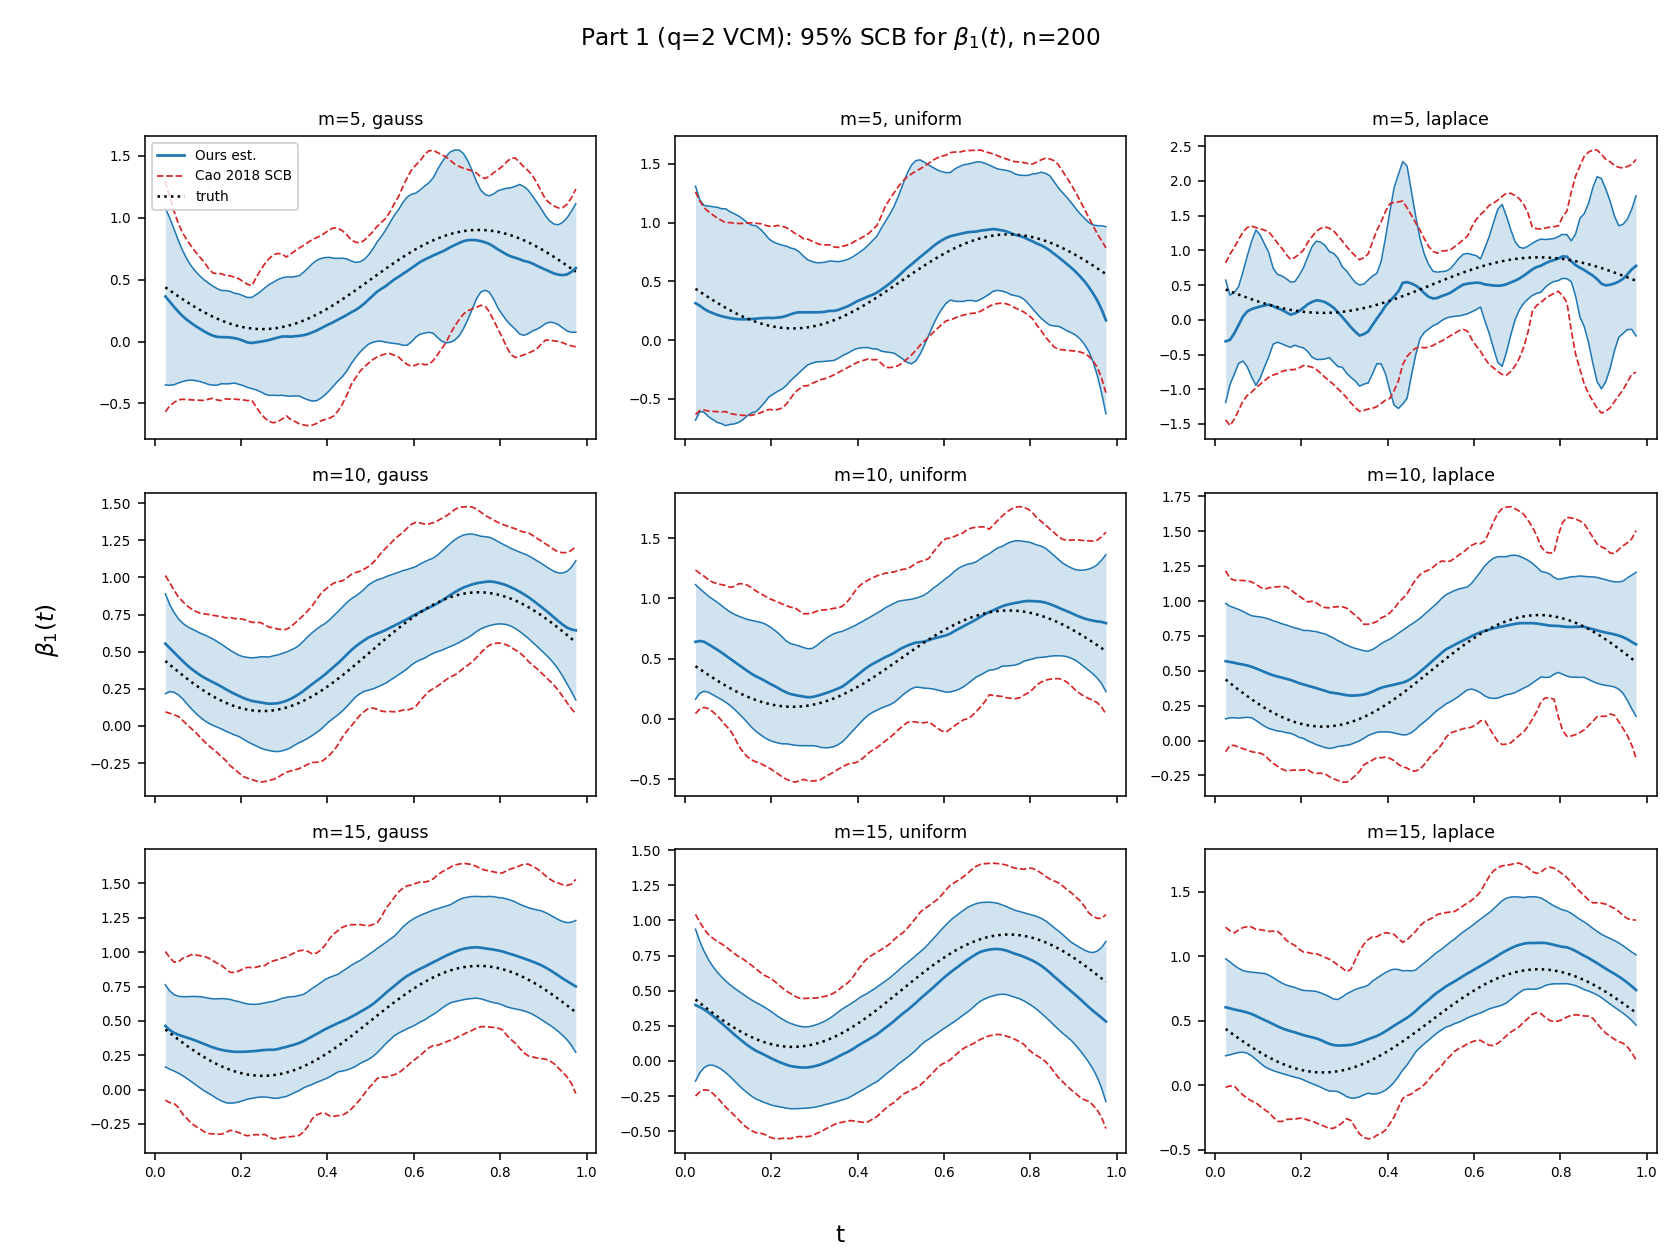
\includegraphics[width=0.48\linewidth]{results/figures/part1_bands_n200.png}
\hfill
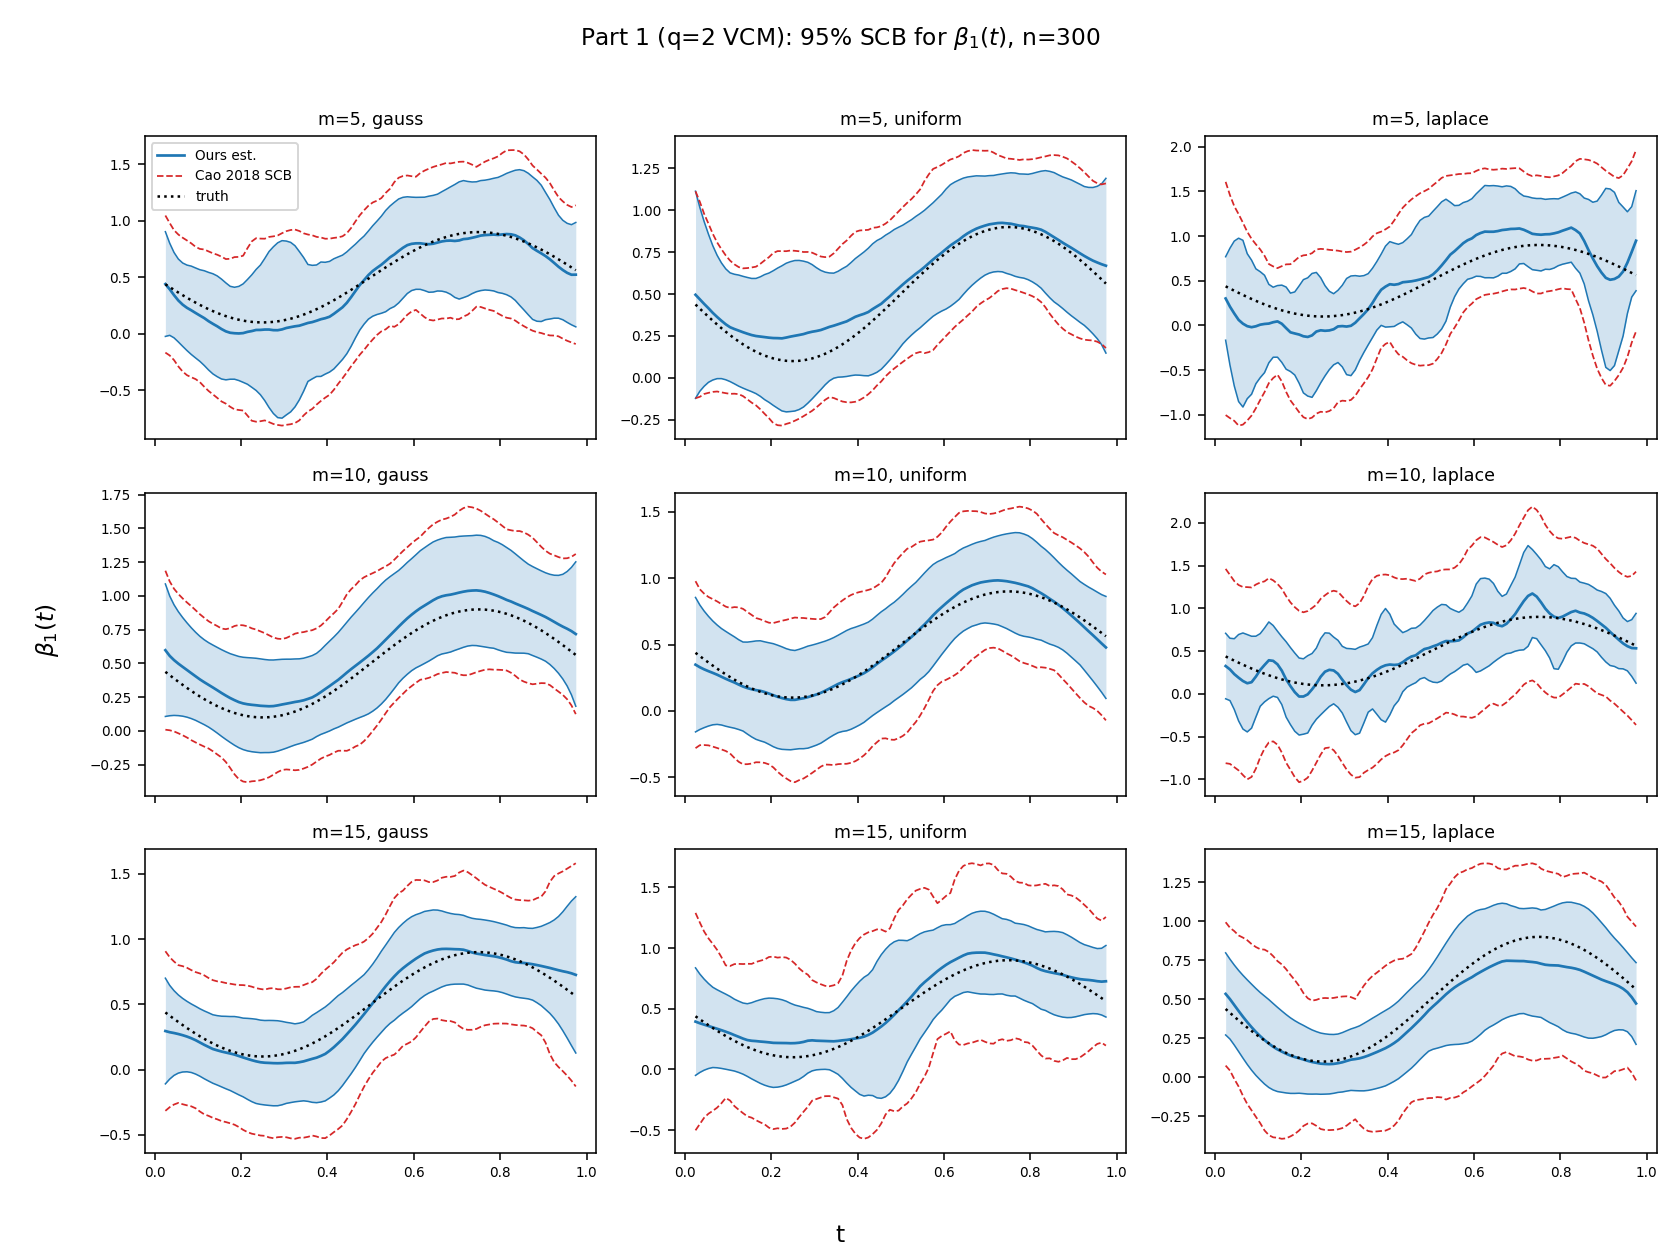
\includegraphics[width=0.48\linewidth]{results/figures/part1_bands_n300.png}
\end{center}
\caption{Representative Part 1 bands for the single-coefficient VCM at
\(n=200\) and \(n=300\). The figure is used only as a one-run illustration;
the tables report Monte Carlo performance.}
\label{fig:part1-bands}
\end{figure}

\begin{table}[t!]
\caption{Part 1, \(n=200\): empirical simultaneous coverage and average band
width for \(\beta_1\). The width ratio is the average width of the proposed
band divided by that of Cao's band.}
\label{tab:part1-200}\par
\resizebox{\linewidth}{!}{%
\begin{tabular}{|ccccc c|}
\hline
$n$ & $m$ & noise & Cao cov/wid & {\bf Ours cov/wid} & width ratio \\
\hline
200 & 5  & gauss   & 0.990/1.385 & {\bf 0.953/1.100} & 0.79 \\
200 & 5  & uniform & 0.984/1.412 & {\bf 0.935/1.126} & 0.80 \\
200 & 5  & laplace & 0.992/1.348 & {\bf 0.949/1.066} & 0.79 \\
200 & 10 & gauss   & 1.000/1.408 & {\bf 0.947/0.860} & 0.61 \\
200 & 10 & uniform & 0.999/1.466 & {\bf 0.944/0.888} & 0.61 \\
200 & 10 & laplace & 0.999/1.389 & {\bf 0.935/0.841} & 0.61 \\
200 & 15 & gauss   & 1.000/1.462 & {\bf 0.937/0.789} & 0.54 \\
200 & 15 & uniform & 0.999/1.461 & {\bf 0.931/0.791} & 0.54 \\
200 & 15 & laplace & 1.000/1.424 & {\bf 0.954/0.764} & 0.54 \\
\hline
\end{tabular}}
\end{table}

\begin{table}[t!]
\caption{Part 1, \(n=300\): empirical simultaneous coverage and average band
width for \(\beta_1\). The width ratio is the average width of the proposed
band divided by that of Cao's band.}
\label{tab:part1-300}\par
\resizebox{\linewidth}{!}{%
\begin{tabular}{|ccccc c|}
\hline
$n$ & $m$ & noise & Cao cov/wid & {\bf Ours cov/wid} & width ratio \\
\hline
300 & 5  & gauss   & 0.991/1.163 & {\bf 0.950/0.871} & 0.75 \\
300 & 5  & uniform & 0.987/1.156 & {\bf 0.947/0.876} & 0.76 \\
300 & 5  & laplace & 0.996/1.104 & {\bf 0.962/0.835} & 0.76 \\
300 & 10 & gauss   & 0.999/1.183 & {\bf 0.941/0.698} & 0.59 \\
300 & 10 & uniform & 0.999/1.175 & {\bf 0.931/0.701} & 0.60 \\
300 & 10 & laplace & 0.999/1.163 & {\bf 0.951/0.684} & 0.59 \\
300 & 15 & gauss   & 1.000/1.181 & {\bf 0.958/0.633} & 0.54 \\
300 & 15 & uniform & 0.999/1.201 & {\bf 0.942/0.640} & 0.53 \\
300 & 15 & laplace & 1.000/1.181 & {\bf 0.950/0.624} & 0.53 \\
\hline
\end{tabular}}
\end{table}

The proposed SCB exhibits stable calibration across all combinations of
\((n,m,\zeta)\). Its empirical coverage ranges from 0.931 to 0.962, with mean
coverage 0.945 and mean absolute deviation from the nominal level equal to
0.008. Cao's plug-in SCB is more conservative, with mean coverage 0.996 and
no configuration below 0.984, and this should be read in light of its target:
it is a sparse-longitudinal-data procedure calibrated through large-sample
extreme-value theory. In the present finite-sample settings, especially as
\(m\) increases, that limiting calibration leads to wider bands than are
needed for nominal coverage. The proposed bands are shorter in every setting,
with average width ratio 0.64 over all 18 configurations; the gain increases
from about 22\% shorter at \(m=5\) to about 47\% shorter at \(m=15\).

\emph{Part 2: joint VCM inference over five coefficients.}
The second experiment moves from a single target curve to joint simultaneous
inference in a
five-dimensional VCM. The coefficient functions are
\[
\beta_0(t)=1,\qquad
\beta_1(t)=2\sin(2\pi t),\qquad
\beta_2(t)=2(t-0.5),
\]
\[
\beta_3(t)=e^t,\qquad
\beta_4(t)=\cos(5\pi t).
\]
The covariate processes are generated from Karhunen--Lo\`eve-type
subject-specific loadings. To check robustness beyond a single error law, we
use standardized Gaussian, uniform, and Laplace observation noise, with the
variance in each case calibrated to yield signal-to-noise ratio 5. The target event is
joint simultaneous coverage:
\[
\beta_k(t)\in[\hat L_k(t),\hat U_k(t)]
\quad \text{for all } k=0,\ldots,4
\text{ and all } t \text{ in the grid}.
\]
Accordingly, the multiplier-bootstrap critical value is computed from the
supremum over the full index set \((k,t)\).

\begin{figure}[t!]
\begin{center}
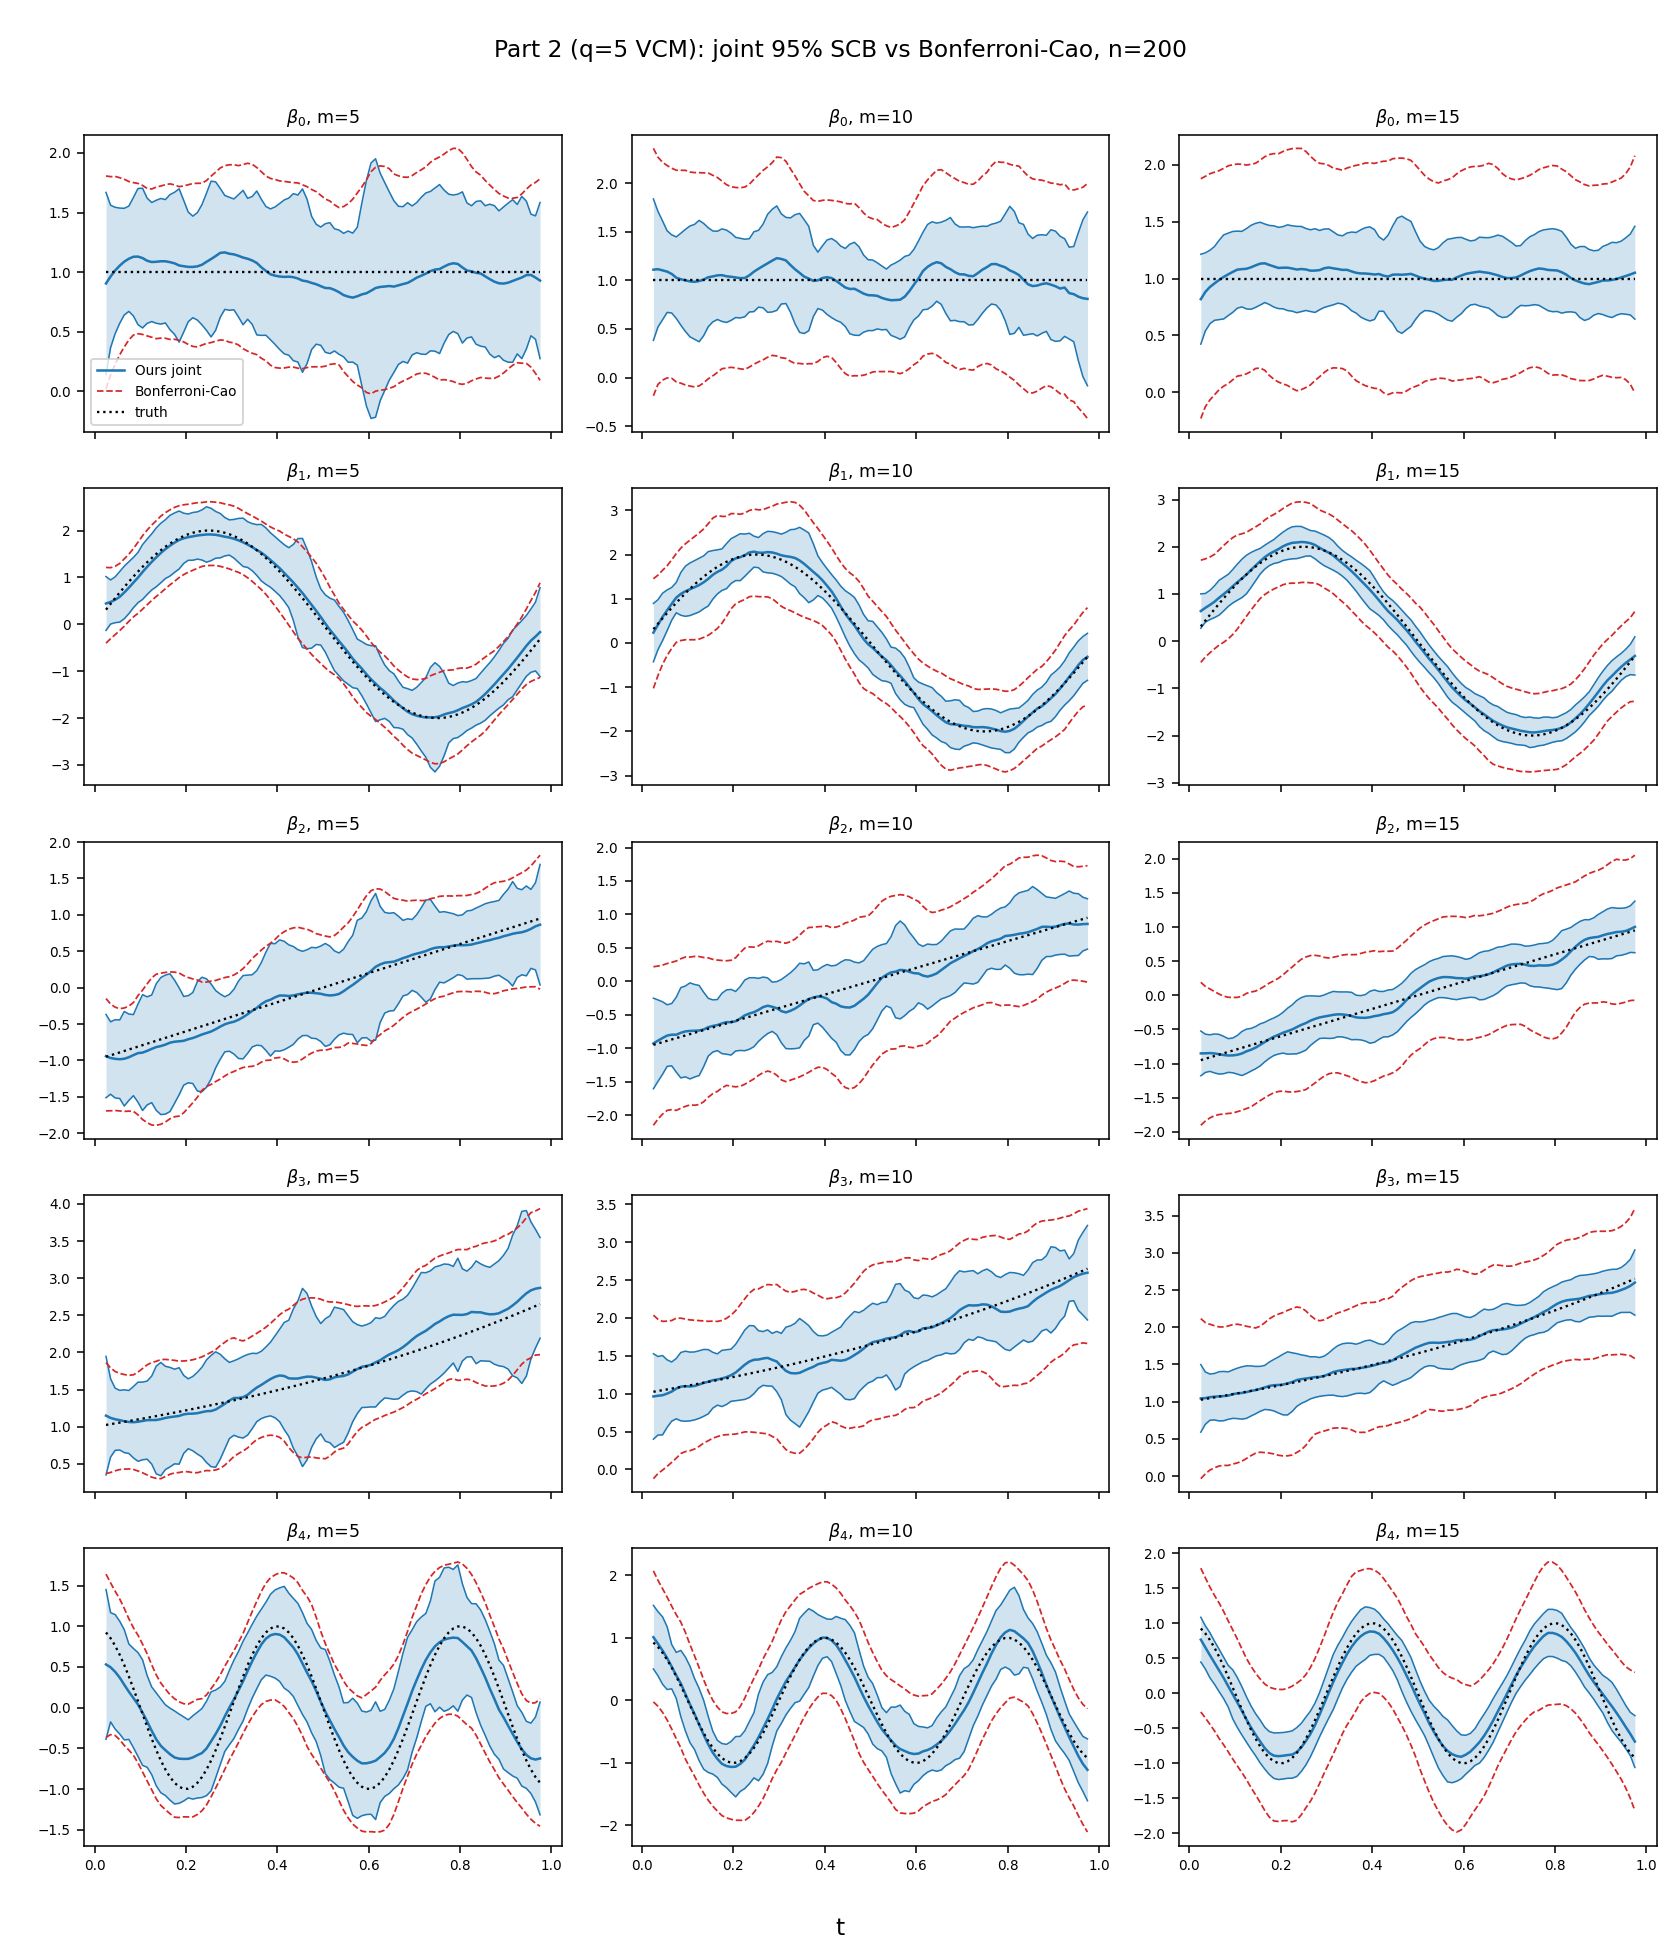
\includegraphics[width=\linewidth]{results/figures/part2_bands_joint.png}
\end{center}
\caption{Representative Part 2 joint bands over the five VCM coefficient
functions. The display illustrates a single simulated dataset; joint
simultaneous coverage is evaluated in Tables~\ref{tab:part2-200}
and~\ref{tab:part2-300}.}
\label{fig:part2-bands}
\end{figure}

The settings are \(n\in\{200,300\}\), \(m\in\{5,10,15\}\), three noise
distributions, and \(R=1{,}000\) replications per configuration. Since Cao's
plug-in SCB is a marginal, per-target
construction, we form a simultaneous benchmark by applying a Bonferroni
correction: each coefficient function is assigned a Cao SCB at level
\(\alpha/p=0.01\), and the intersection of the five bands is used as the joint
SCB.

\begin{table}[t!]
\caption{Part 2, \(n=200\): joint simultaneous coverage over all five
coefficient functions. Width is averaged over the five components.}
\label{tab:part2-200}\par
\begin{center}
\begin{tabular}{|ccccc|}
\hline
\(m\) & Noise & {\bf Ours cov/wid} & Bonferroni--Cao cov/wid & ratio \\
\hline
5  & Gaussian & {\bf 0.967}/1.340 & 1.000/1.617 & 0.83 \\
5  & Uniform  & {\bf 0.964}/1.354 & 1.000/1.622 & 0.84 \\
5  & Laplace  & {\bf 0.955}/1.322 & 1.000/1.605 & 0.82 \\
10 & Gaussian & {\bf 0.960}/0.849 & 1.000/1.775 & 0.48 \\
10 & Uniform  & {\bf 0.962}/0.856 & 1.000/1.782 & 0.48 \\
10 & Laplace  & {\bf 0.962}/0.845 & 1.000/1.770 & 0.48 \\
15 & Gaussian & {\bf 0.960}/0.680 & 1.000/1.863 & 0.37 \\
15 & Uniform  & {\bf 0.962}/0.683 & 1.000/1.866 & 0.37 \\
15 & Laplace  & {\bf 0.949}/0.678 & 1.000/1.861 & 0.36 \\
\hline
\end{tabular}
\end{center}
\end{table}

\begin{table}[t!]
\caption{Part 2, \(n=300\): joint simultaneous coverage over all five
coefficient functions. Width is averaged over the five components.}
\label{tab:part2-300}\par
\begin{center}
\begin{tabular}{|ccccc|}
\hline
\(m\) & Noise & {\bf Ours cov/wid} & Bonferroni--Cao cov/wid & ratio \\
\hline
5  & Gaussian & {\bf 0.950}/0.969 & 1.000/1.365 & 0.71 \\
5  & Uniform  & {\bf 0.967}/0.971 & 1.000/1.364 & 0.71 \\
5  & Laplace  & {\bf 0.958}/0.955 & 1.000/1.353 & 0.71 \\
10 & Gaussian & {\bf 0.938}/0.650 & 1.000/1.505 & 0.43 \\
10 & Uniform  & {\bf 0.943}/0.655 & 1.000/1.515 & 0.43 \\
10 & Laplace  & {\bf 0.942}/0.648 & 1.000/1.503 & 0.43 \\
15 & Gaussian & {\bf 0.941}/0.531 & 1.000/1.578 & 0.34 \\
15 & Uniform  & {\bf 0.947}/0.533 & 1.000/1.582 & 0.34 \\
15 & Laplace  & {\bf 0.938}/0.531 & 1.000/1.579 & 0.34 \\
\hline
\end{tabular}
\end{center}
\end{table}

Tables~\ref{tab:part2-200} and~\ref{tab:part2-300} show that the proposed
joint SCB remains stable over the full grid of sample sizes, sampling
densities, and noise distributions. Across the 18 configurations, its empirical
coverage ranges from 0.938 to 0.967, with mean coverage 0.954. This is close to
the nominal level for a band that must cover five coefficient functions
simultaneously over the whole time grid. The average width also decreases
systematically as the within-subject sampling density increases: averaging over
\(n\) and the noise laws, the width falls from 1.152 at \(m=5\) to 0.750 at
\(m=10\) and 0.606 at \(m=15\).

The Bonferroni-adjusted Cao benchmark also attains simultaneous coverage, but
does so conservatively. This is not surprising: a marginal sparse-design band,
already based on an extreme-value approximation, is being asked to deliver a
joint five-function statement after Bonferroni inflation. Its empirical
coverage is 1.000 in all 18 settings, while its mean width is nearly twice that
of the proposed band. The relative gain is most visible as \(m\) increases:
averaged over \(n\) and the noise distributions, the proposed joint band uses
about 77\%, 46\%, and 35\% of the Bonferroni--Cao width at \(m=5,10,15\),
respectively. The comparison therefore mainly illustrates the cost of
converting a marginal sparse-data procedure into a genuinely joint
multi-coefficient band.

\emph{Part 3: mean function inference.}
The third experiment considers SCB construction for a mean function under a
standard sparse functional data model. The data are generated from
\begin{equation}
\label{eq:part3-dgp}
Y_{ij}=m(T_{ij})+\phi(T_{ij})^\top\xi_i+
\sigma_\varepsilon\varepsilon_{ij},
\end{equation}
where
\[
m(t)=1.5\sin\{3\pi(t+0.5)\}+2t^3,
\]
\[
\phi(t)=\sqrt2(\sin2\pi t,\cos2\pi t,\sin4\pi t,\cos4\pi t).
\]
The associated eigenvalues are \((1,1/2,1/4,1/8)\), and
\(\sigma_\varepsilon=0.1\). The random variables \(\xi_i\) and
\(\varepsilon_{ij}\) are generated independently from one of three
unit-variance distributions: \(N(0,1)\),
\(\mathrm{Uniform}(-\sqrt3,\sqrt3)\), or
\(\mathrm{Laplace}(0,1/\sqrt2)\).

The simulation settings are \(n\in\{200,300\}\),
\(m\in\{5,10,15\}\), and the three error distributions, again giving 18
configurations in total. The proposed local-linear SCB is compared with the
B-spline SCB of \citet{CaiHu2025}.

\begin{figure}[t!]
\begin{center}
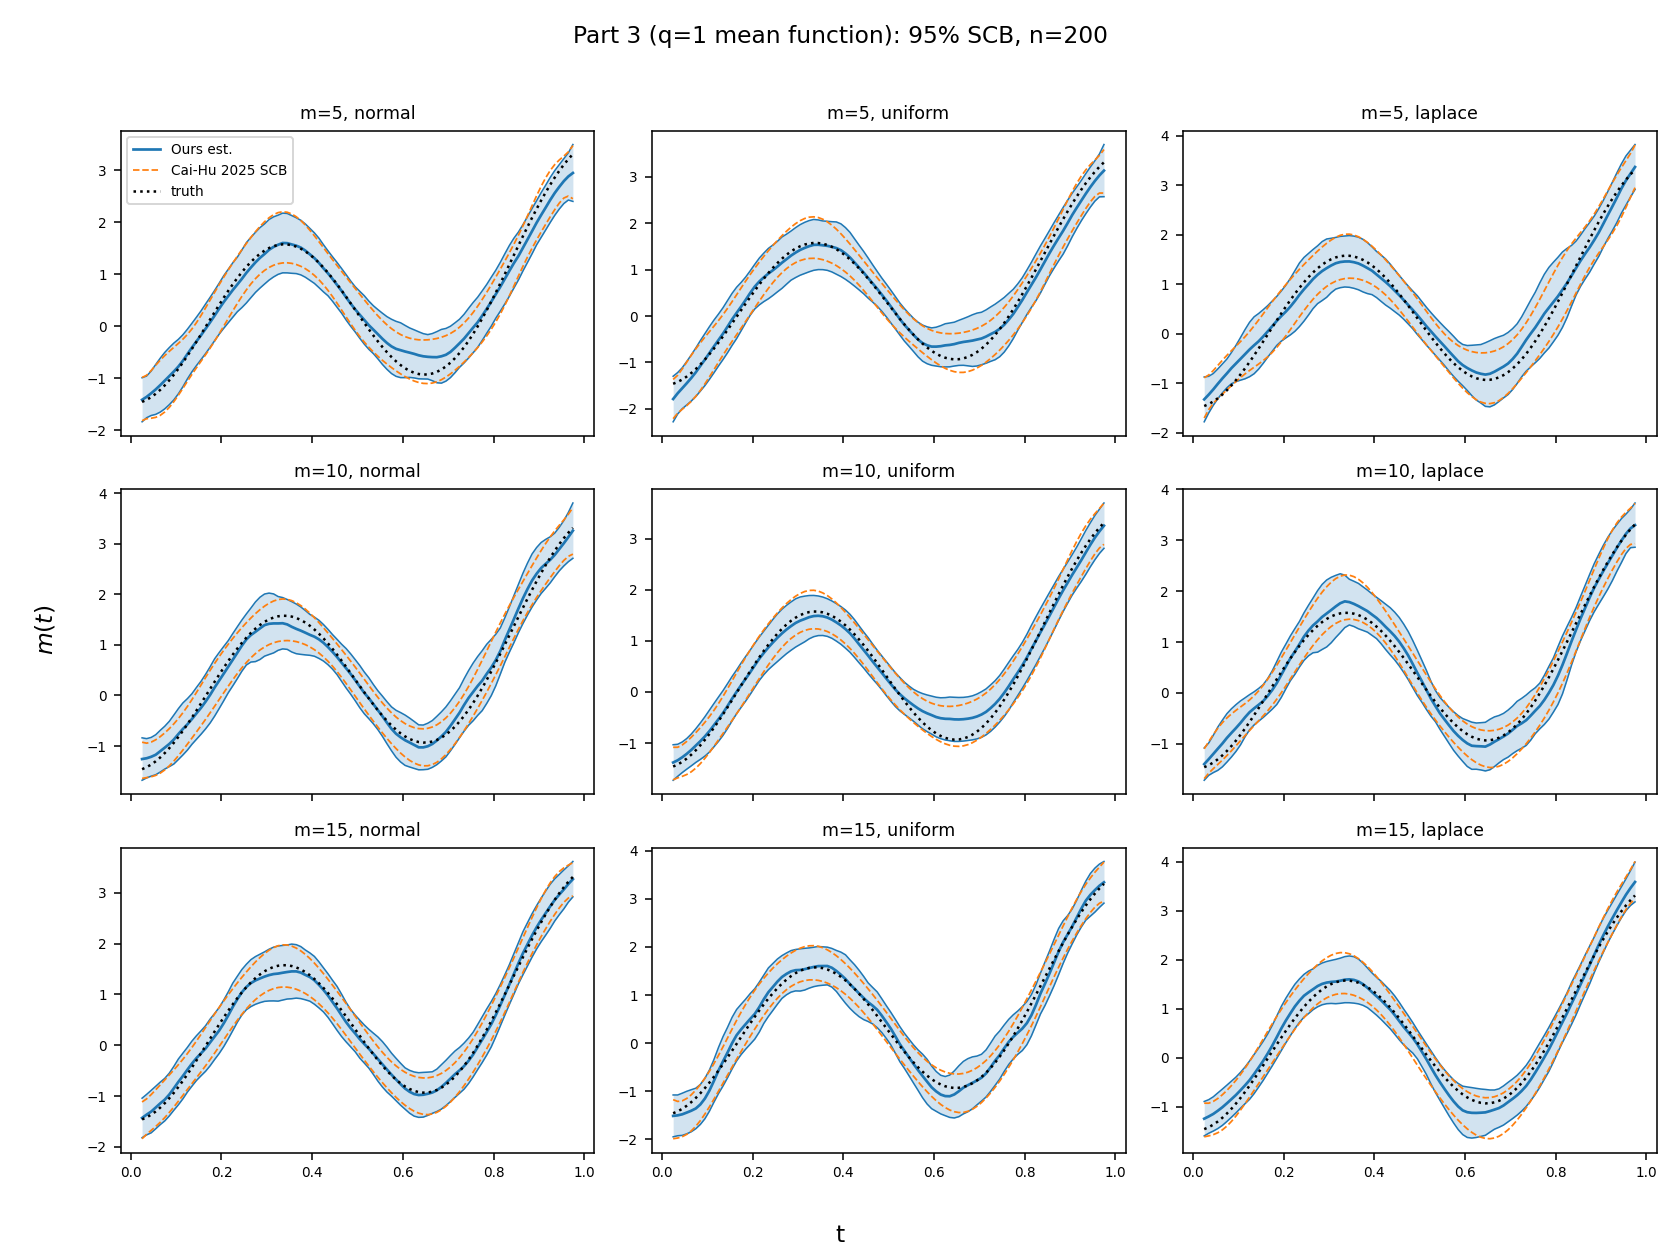
\includegraphics[width=0.48\linewidth]{results/figures/part3_bands_n200.png}
\hfill
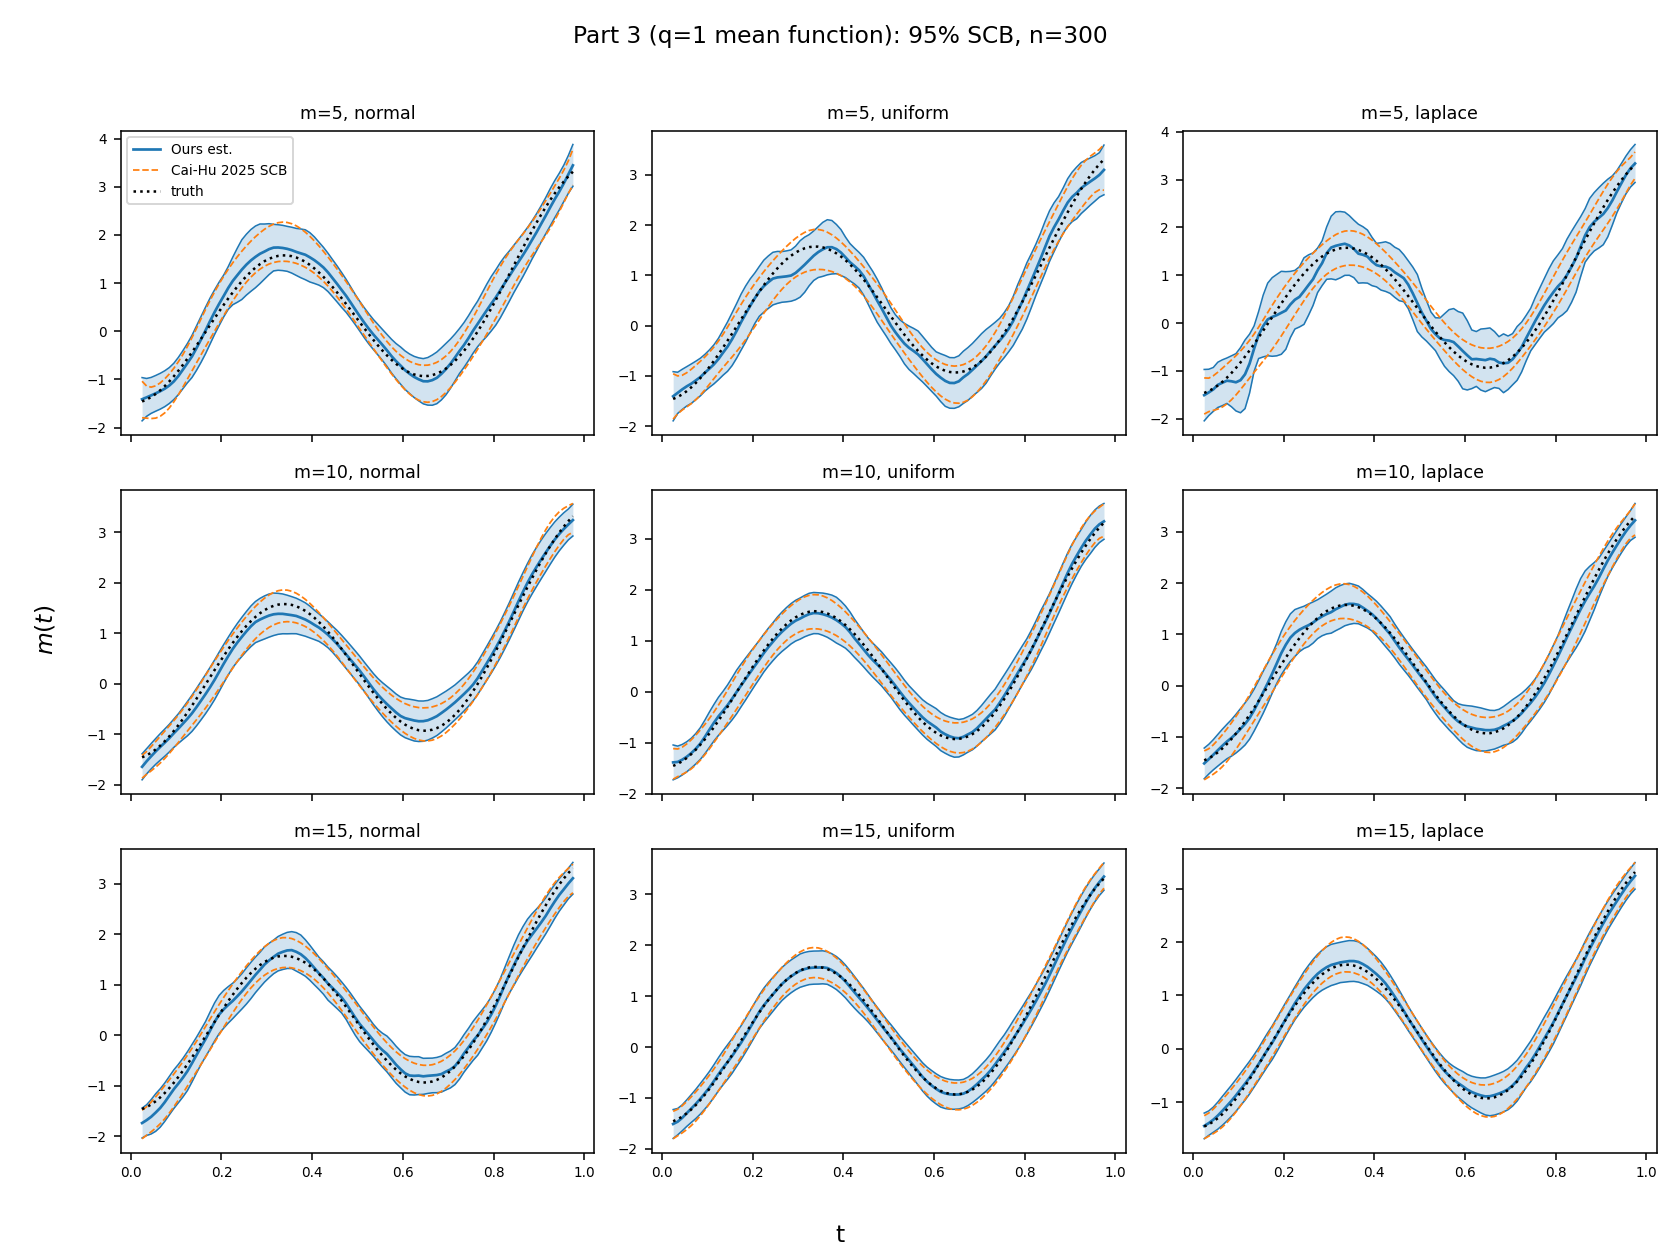
\includegraphics[width=0.48\linewidth]{results/figures/part3_bands_n300.png}
\end{center}
\caption{Representative Part 3 bands for mean-function inference at
\(n=200\) and \(n=300\). As in the preceding figures, these are single-run
illustrations, while Tables~\ref{tab:part3-200}--\ref{tab:part3-300}
summarize repeated-sampling behavior.}
\label{fig:part3-bands}
\end{figure}

\begin{table}[t!]
\caption{Part 3: mean function SCB, comparing the proposed band with the
Cai--Hu (2025) B-spline band for \(n=200\).}
\label{tab:part3-200}\par
\resizebox{\linewidth}{!}{%
\begin{tabular}{|ccccc|}
\hline
$n$ & $m$ & noise & {\bf Ours cov/wid} & Cai--Hu cov/wid \\
\hline
200 & 5  & normal  & {\bf 0.965/1.115} & 0.919/0.892 \\
200 & 5  & uniform & {\bf 0.961/1.122} & 0.908/0.893 \\
200 & 5  & laplace & {\bf 0.957/1.111} & 0.906/0.889 \\
200 & 10 & normal  & {\bf 0.960/0.889} & 0.936/0.743 \\
200 & 10 & uniform & {\bf 0.959/0.890} & 0.931/0.742 \\
200 & 10 & laplace & {\bf 0.953/0.886} & 0.931/0.741 \\
200 & 15 & normal  & {\bf 0.951/0.806} & 0.927/0.685 \\
200 & 15 & uniform & {\bf 0.959/0.805} & 0.930/0.686 \\
200 & 15 & laplace & {\bf 0.947/0.800} & 0.941/0.682 \\
\hline
\end{tabular}}
\end{table}

\begin{table}[t!]
\caption{Part 3: mean function SCB, comparing the proposed band with the
Cai--Hu (2025) B-spline band for \(n=300\).}
\label{tab:part3-300}\par
\resizebox{\linewidth}{!}{%
\begin{tabular}{|ccccc|}
\hline
$n$ & $m$ & noise & {\bf Ours cov/wid} & Cai--Hu cov/wid \\
\hline
300 & 5  & normal  & {\bf 0.949/0.896} & 0.922/0.732 \\
300 & 5  & uniform & {\bf 0.954/0.901} & 0.923/0.733 \\
300 & 5  & laplace & {\bf 0.958/0.896} & 0.927/0.730 \\
300 & 10 & normal  & {\bf 0.941/0.728} & 0.928/0.609 \\
300 & 10 & uniform & {\bf 0.958/0.731} & 0.934/0.608 \\
300 & 10 & laplace & {\bf 0.948/0.730} & 0.920/0.608 \\
300 & 15 & normal  & {\bf 0.957/0.661} & 0.923/0.561 \\
300 & 15 & uniform & {\bf 0.943/0.661} & 0.916/0.561 \\
300 & 15 & laplace & {\bf 0.958/0.658} & 0.946/0.559 \\
\hline
\end{tabular}}
\end{table}

Tables~\ref{tab:part3-200} and~\ref{tab:part3-300} show that the proposed
SCB is well calibrated in the mean-function setting. Across all 18
configurations, its empirical coverage ranges from 0.941 to 0.965, with mean
coverage 0.954 and mean absolute deviation from the nominal level equal to
0.007. The Cai--Hu B-spline SCB is uniformly narrower, with mean width 0.703
compared with 0.849 for the proposed method, and its coverage remains broadly
reasonable for a finite-sample comparison. Its mean coverage is 0.926, so the
main difference is the familiar efficiency-calibration trade-off: the
specialized B-spline construction gives shorter bands, whereas the proposed
local-linear procedure stays closer to the nominal simultaneous level while
using the same algorithm as in the VCM experiments.

Taken together, the simulations show that the proposed SCB is stable across
the settings considered. It performs consistently for a marginal VCM target,
continues to work when the inferential target becomes genuinely
multi-dimensional and simultaneous, and remains effective when the same
construction is applied to mean-function inference. This stability, rather
than a scenario-specific tuning advantage, is the main numerical message.

\subsection{Real data application: Mayo PBC sequential biomarkers}
\label{subsec:realdata}

We apply the proposed SCB to the Mayo PBC sequential biomarker dataset
\citep{TherneauGrambsch2000}, available as \texttt{pbcseq} in the R
\texttt{survival} package. The data arise from the Mayo Clinic randomized
D-penicillamine trial for primary biliary cirrhosis (PBC) reported by
\citet{Dickson1985}. The full
longitudinal record contains 1,945 serial measurements from \(n=312\) patients,
with follow-up extending to approximately 13 years. We restrict attention to
the first 8.2 years, corresponding to \(\mathrm{day}\le 3{,}000\), which
retains approximately 92\% of the observations. After excluding records with
missing bilirubin values, the analysis sample consists of 1,790 observations
from all 312 patients.

\begin{figure}[t!]
\centerline{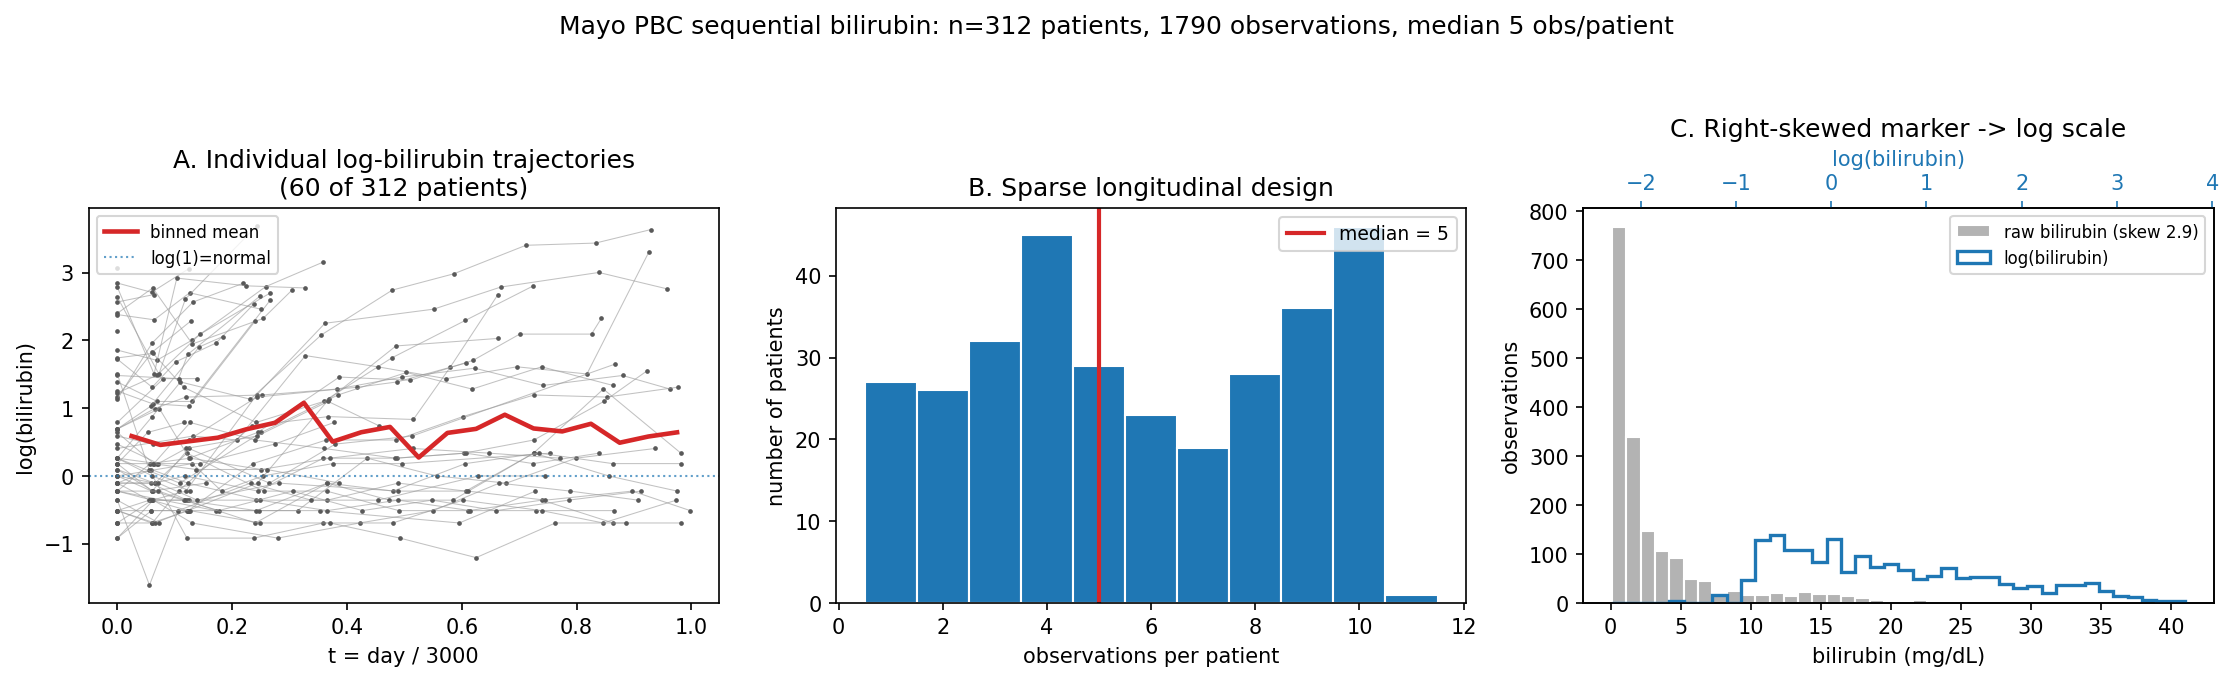
\includegraphics[width=\linewidth]{results/realdata/pbc_data_illustration.png}}
\caption{Mayo PBC design illustration: individual log-bilirubin trajectories,
the distribution of repeated measurements per patient, and the marginal
distribution of raw bilirubin.}
\label{fig:pbc-data}
\end{figure}

Figure~\ref{fig:pbc-data} summarizes the longitudinal design. Measurements are
taken at irregular, patient-specific visit times, with a median of 5
observations per patient, a mean of 5.7, and a range of 1--11. The data
therefore constitute a sparse longitudinal design, consistent with the
sampling regimes considered in the simulation study. The raw bilirubin
measurements are strongly right-skewed, with sample skewness 2.88; following
standard analyses of this dataset \citep{TherneauGrambsch2000},
we analyze \(\log(\mathrm{bilirubin})\) and rescale time as
\(t=\mathrm{day}/3000\in[0,1]\) for kernel estimation. The treatment arms are
nearly balanced, with 158 patients assigned to D-penicillamine and 154 assigned
to placebo.

The biological question is not merely whether a smooth curve can be estimated.
PBC is a chronic cholestatic liver disease in which progressive bile-duct
injury can be reflected in rising bilirubin and alkaline phosphatase, while
impaired liver synthetic function is reflected by lower albumin and longer
prothrombin time \citep{KaplanGershwin2005,Lindor2019}. Bilirubin is also a
central prognostic marker in the Mayo PBC literature
\citep{Dickson1989,Murtaugh1994}. Thus the data allow two linked questions:
first, whether the cohort shows a population-level bilirubin elevation over
follow-up; and second, whether the time-varying bilirubin trajectory is more
closely associated with the randomized D-penicillamine assignment or with
contemporaneous markers of cholestasis and hepatic decompensation.

\emph{Mean trajectory.}
We begin with the population mean, since it gives the clinical scale of the
phenomenon before covariates are introduced. The mean-function model is
\begin{equation}
\label{eq:pbc-mean-model}
\log(\mathrm{bili}_{ij})=m(t_{ij})+\varepsilon_{ij}.
\end{equation}

For this model, the data-driven bandwidth selection gives
\(\hat h_{\mathrm{est}}=0.160\) and \(\hat h_{\mathrm{inf}}=0.113\). The
bootstrap critical value is \(\hat q_{\mathrm{crit}}=2.81\), and the average
SCB width on the log scale is 0.55. For comparison, the Cai--Hu B-spline SCB
selects \(J_n=6\) interior knots and has average width 0.56, so the two
real-data mean bands are very similar in overall width; the width ratio of the
proposed band relative to the B-spline band is 0.97.
Figure~\ref{fig:pbc-mean} displays the estimated trajectory and SCB on both
the log scale and the back-transformed clinical scale, while
Table~\ref{tab:pbc-mean} reports selected values on the clinical scale.

\begin{figure}[t!]
\centerline{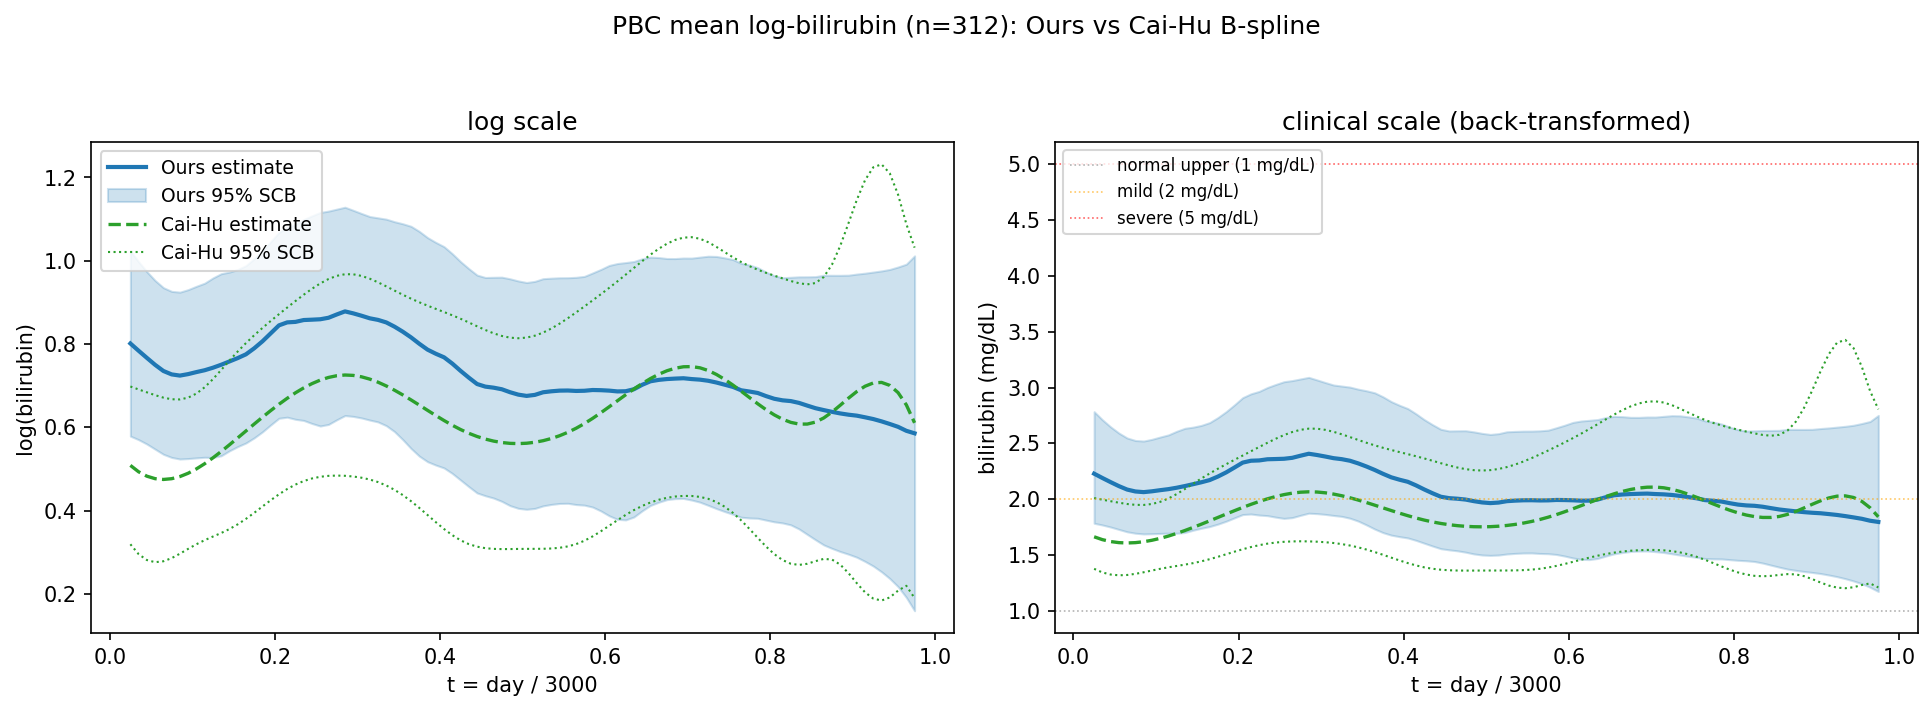
\includegraphics[width=\linewidth]{results/realdata/pbc_mean_bands.png}}
\caption{PBC mean bilirubin trajectory with simultaneous confidence bands on
the log scale and on the back-transformed clinical scale.}
\label{fig:pbc-mean}
\end{figure}

\begin{table}[t!]
\caption{PBC mean bilirubin, back-transformed to mg/dL, with the 95\% SCB at
selected follow-up times.}
\label{tab:pbc-mean}\par
\begin{center}
\begin{tabular}{|lcc|}
\hline
Time & $\widehat m(t)$ as bili (mg/dL) & 95\% SCB (mg/dL) \\
\hline
day 135  ($t=0.04$) & 2.15 & $[1.75,2.65]$ \\
day 795  ($t=0.27$) & 2.37 & $[1.83,3.06]$ \\
day 1545 ($t=0.52$) & 1.97 & $[1.50,2.59]$ \\
day 2235 ($t=0.74$) & 2.02 & $[1.49,2.74]$ \\
day 2865 ($t=0.95$) & 1.82 & $[1.24,2.68]$ \\
\hline
\end{tabular}
\end{center}
\end{table}

The estimated mean trajectory is above the normal reference value of
1.0 mg/dL at the selected time points in Table~\ref{tab:pbc-mean}; the lower
SCB endpoints are also above this threshold. This provides simultaneous
population-level evidence of hyperbilirubinemia in the Mayo PBC cohort, in
line with the role of bilirubin as a marker of advanced disease
\citep{Dickson1989,Prince2004,Corpechot2008}. The curve rises during early
follow-up, reaching about 2.4 mg/dL around day 800, and then remains near
2.0 mg/dL through the middle and later portions of the observed window. We do
not interpret the modest flattening and later decline as a typical
within-patient recovery pattern. In a longitudinal PBC cohort, the sickest
patients may die, receive transplantation, or otherwise leave follow-up earlier;
the later cross-sectional mean is therefore computed among a selected set of
survivors \citep{Murtaugh1994,WulfsohnTsiatis1997}. The SCB is valuable here
because it turns this visual impression into a simultaneous statement about
the population trajectory over the observed follow-up window.

\emph{Varying-coefficient analysis.}
The mean analysis establishes that bilirubin is elevated at the cohort level,
but it does not distinguish between treatment assignment and the biological
state of the liver. We therefore turn to a varying-coefficient model that
includes the randomized D-penicillamine indicator and clinically interpretable
markers of decompensation and cholestasis. The outcome remains
\(\log(\mathrm{bilirubin})\), and the covariates are treatment, edema score,
albumin, prothrombin time, and \(\log(\mathrm{alkaline\ phosphatase})\). Edema,
albumin, and prothrombin time are part of the classical Mayo prognostic
framework \citep{Dickson1989,Murtaugh1994}, while alkaline phosphatase is a
standard cholestatic marker in PBC assessment and risk stratification
\citep{Lindor2019,Lammers2014,Carbone2016}. After excluding records with
missing alkaline phosphatase, this analysis uses 1,741 observations from all
312 patients. The non-binary covariates are centered and scaled, so their
coefficients are interpreted per one-standard-deviation increase. The model is
\begin{equation}
\label{eq:pbc-vcm-model}
\begin{split}
\log(\mathrm{bili}_{ij})
=&\,\beta_0(t_{ij})+\beta_1(t_{ij})\mathrm{trt}_i
 +\beta_2(t_{ij})\mathrm{edema}^{\mathrm{std}}_{ij} \\
&+\beta_3(t_{ij})\mathrm{albumin}^{\mathrm{std}}_{ij}
 +\beta_4(t_{ij})\mathrm{protime}^{\mathrm{std}}_{ij} \\
&+\beta_5(t_{ij})\log(\mathrm{ALP}_{ij})^{\mathrm{std}}
 +\varepsilon_{ij},
\end{split}
\end{equation}
where \(\mathrm{trt}_i=1\) denotes assignment to D-penicillamine.

Because inference is required for six coefficient functions over a continuum of
time points, we report a joint SCB over all components. The bootstrap supremum
is taken jointly over both coefficient index and time, so that the resulting
band targets
\[
P\{\hat L_k(t)\le\beta_k(t)\le\hat U_k(t)\ {\rm for\ all}\ k,t\}
\approx0.95.
\]
For this joint model, the data-driven bandwidth selection gives
\(\hat h_{\mathrm{est}}=0.160\) and \(\hat h_{\mathrm{inf}}=0.086\). The
joint bootstrap critical value is
\(\hat q_{\mathrm{crit}}^{\mathrm{joint}}=3.59\). For reference, we also report
the marginal Cao plug-in SCB, for which the critical constant is
\(\gamma=2.82\). The resulting bands are displayed in
Figure~\ref{fig:pbc-vcm}.

\begin{figure}[t!]
\centerline{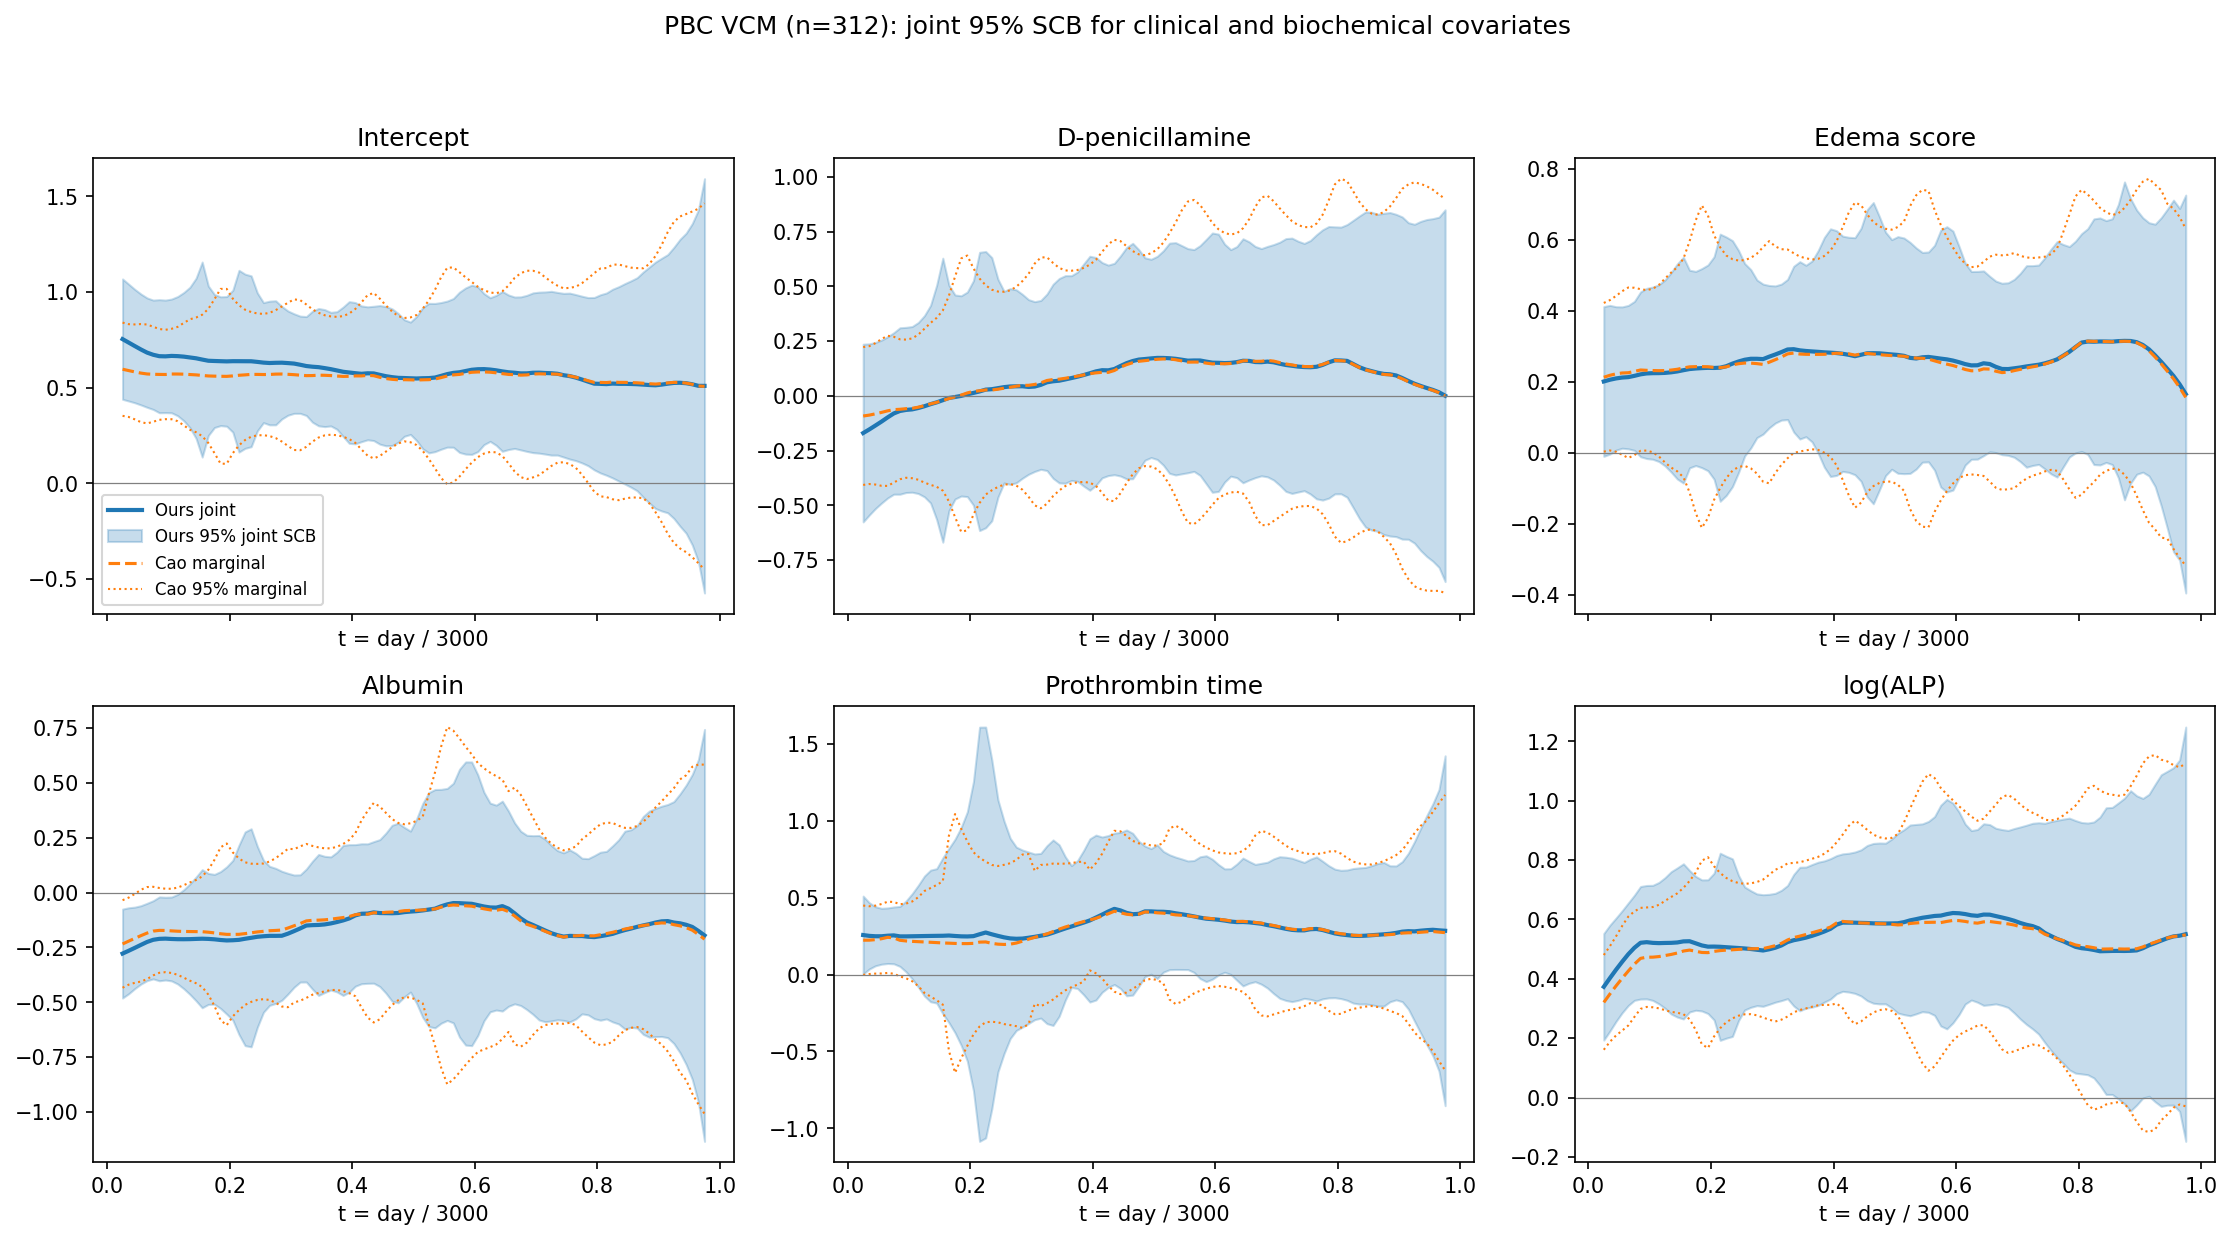
\includegraphics[width=\linewidth]{results/realdata/pbc_vcm_bands.png}}
\caption{PBC varying-coefficient analysis: joint 95\% SCB for treatment,
edema, albumin, prothrombin time, and log alkaline phosphatase effects.}
\label{fig:pbc-vcm}
\end{figure}

\begin{table}[t!]
\caption{PBC VCM analysis: proposed joint 95\% SCB versus the marginal Cao
band. The final column records whether the proposed joint band excludes zero
over at least one time interval.}
\label{tab:pbc-vcm}\par
\resizebox{\linewidth}{!}{%
\begin{tabular}{|lcccc|}
\hline
Coefficient & Ours joint wid & Cao wid & width ratio & Joint band excludes 0? \\
\hline
$\beta_0$ (intercept)                & 0.837 & 0.902 & 0.93 & yes \\
$\beta_1$ (D-penicillamine)          & 1.082 & 1.192 & 0.91 & no \\
$\beta_2$ (edema)                    & 0.613 & 0.689 & 0.89 & yes \\
$\beta_3$ (albumin)                  & 0.794 & 0.882 & 0.90 & yes \\
$\beta_4$ (prothrombin time)         & 1.001 & 0.973 & 1.03 & yes \\
$\beta_5$ (log alkaline phosphatase) & 0.632 & 0.706 & 0.89 & yes \\
\hline
\end{tabular}}
\end{table}

The VCM analysis gives a sharper biological interpretation of the elevated
mean trajectory. The D-penicillamine band contains zero over the entire
follow-up window, consistent with the original trial conclusion that
D-penicillamine did not provide a meaningful clinical benefit in advanced PBC
\citep{Dickson1985,Lindor2009,Lindor2019}. By contrast, the log alkaline
phosphatase coefficient is positive over most of the interior time range,
indicating that higher cholestatic burden is associated with higher
log-bilirubin even after joint simultaneous adjustment for the other clinical
markers. This direction agrees with large PBC cohorts showing that alkaline
phosphatase and bilirubin jointly summarize cholestatic disease activity and
long-term outcome risk \citep{Lammers2014,Carbone2016}. The edema and
prothrombin-time coefficients are also positive over selected intervals, while
the albumin coefficient is negative early in follow-up. These signs are
biologically coherent and are supported by the Mayo prognostic literature:
edema and prolonged prothrombin time indicate decompensation and impaired
synthetic function, whereas higher albumin indicates better preserved synthetic
function \citep{Dickson1989,Murtaugh1994,KaplanGershwin2005}. The
comparison with the marginal Cao bands is not the main clinical message, but it
shows that the proposed joint band remains competitive in width: it is shorter
for five of the six coefficients and only slightly wider for prothrombin time,
despite protecting the entire six-function statement simultaneously.

Taken together, the real-data analysis answers the motivating clinical problem
in two stages. The mean SCB shows that the Mayo cohort has a persistently
elevated bilirubin profile on the population scale. The expanded VCM then
shows that the time-varying bilirubin trajectory is not detectably shifted by
D-penicillamine assignment, but is strongly aligned with cholestasis and
hepatic functional status. This is the type of conclusion for which a joint
SCB is useful: it distinguishes a null treatment pattern from several
biologically interpretable marker associations while preserving simultaneous
coverage across functions and time.
